\documentclass{article}
\usepackage[utf8]{inputenc}

\usepackage{amsfonts}
\usepackage{amssymb}
\usepackage{amsmath}
\usepackage{amsthm}
\usepackage{enumitem}

\usepackage{bbold}
\usepackage{bm}
\usepackage{graphicx}
\usepackage{color}
\usepackage{hyperref}
\usepackage[margin=2.5cm]{geometry}

\begin{document}

% ==============================================================================

\title{\Large{INFO8006: Project 2 - Report}}
\vspace{1cm}
\author{}

\maketitle

% ==============================================================================

\section{Bayes filter}

\begin{enumerate}[label=\alph*.,leftmargin=*]
    \item Let $X_t$ be a ghost's cell, $p_t$ Pacman's position,
    and $d(x,p)=|x_1-p_1|+|x_2-p_2|$. For requested variance $v$,
    put $n=\lfloor4v\rfloor$ and $K_t\sim\mathrm{Binomial}(n,1/2)$.
    The measurement is $E_t=d(X_t,p_t)+K_t-n/2$. Therefore, with
    $k=e-d(x,p_t)+n/2$,
    \[
      O(e\mid x,p_t)=
      \begin{cases}\binom{n}{k}2^{-n},& k\in\{0,\ldots,n\},\\
      0,&\text{otherwise.}\end{cases}
    \]
    The sensor is unbiased and its actual variance is $n/4$, which need
    not equal the requested $v$. Measurements can be negative, and are
    half-integers when $n$ is odd. No clipping or rounding is appropriate.
    Wall cells have zero prior mass and zero likelihood in the grid model.

    \item Let $N(x)$ be the free cardinal neighbors of $x$, including the
    reverse direction. Define a single parameter $q\geq0$ and weights
    \[
    w_q(y;x,p)=2^{q\,\mathbb{I}[d(y,p)\geq d(x,p)]},\qquad
    T_q(y\mid x,p)=
      \frac{\mathbb{I}[y\in N(x)]w_q(y;x,p)}
           {\sum_{z\in N(x)}w_q(z;x,p)}.
    \]
    The three policies correspond to $q=0$ (confused), $q=1$ (afraid),
    and $q=3$ (scared). Thus nonapproaching moves receive weights $1,2,8$,
    respectively, and approaching moves receive weight $1$.
    An isolated free cell has a self-transition of probability one.
    This models motion before capture; a known captured ghost is removed
    from the tracking distribution. For each active ghost the recursion is
    \[
    \bar b_t(y)=\sum_x T_q(y\mid x,p_t)b_{t-1}(x),\qquad
    b_t(y)=\frac{O(e_t\mid y,p_t)\bar b_t(y)}
                  {\sum_z O(e_t\mid z,p_t)\bar b_t(z)}.
    \]
\end{enumerate}

\section{Implementation}

\begin{enumerate}[label=\alph*.,leftmargin=*]
    \item \textbf{\textit{Leave empty.}}
\end{enumerate}

\section{Experiment}

\begin{enumerate}[label=\alph*.,leftmargin=*]
    \item Uncertainty is Shannon entropy
    $H(b)=-\sum_{x:b(x)>0}b(x)\log_2b(x)$, measured in bits.
    Zero entropy means certainty; $\log_2M$ is the maximum over $M$ cells.
    Entropy measures confidence, not whether the confidence is correct.
    Active ghosts are averaged within a trial; captured ghosts are excluded.

    \item Quality is the Brier score
    $B(b,x^*)=\sum_x(b(x)-\mathbb{I}[x=x^*])^2$.
    It is zero for correct certainty and approaches two for wrong certainty.
    We also record $\sum_x b(x)d(x,x^*)$ and $b(x^*)$ for diagnostics.
    True positions are used only to compute evaluation metrics.

    \item We ran 30 trials per condition, with
    3 independent ghosts per trial, on both supplied filter layouts.
    Each policy was tested at $v\in\{0.25,1,4\}$, using seed 193611.
    Runs used 1800 steps at $v=0.25,1$ and 9000 steps at $v=4$;
    the longer runs resolve the slower uncertainty decay at high noise.
    The default-variance comparison is $v=1$.
    To avoid early termination and survivor-selection bias, Pacman stays
    at its initial cell and capture is disabled in these controlled tracking
    experiments. Motion probabilities come from the supplied ghost policies
    evaluated through geometric observations without collision side effects;
    they are not sampled from the filter's transition matrix.
    All ghosts move before each sensor update. The submitted filter and
    metric recorder are used unchanged. Separately, live-engine tests run
    the moving bonus controller with capture enabled on both layouts and
    every ghost policy (seeds 1 and 42, three ghosts).

    Each plotted error bar is a pointwise 95\% Student-$t$ confidence interval
    across trial means, not across time steps or individual ghosts.
    The table averages the final 600 steps of each trial.
    \begin{center}
    \begin{tabular}{llcc}
    Layout & Policy & Entropy (bits) & Brier score \\\hline
    Open & confused & $3.347\pm0.033$ & $0.870\pm0.006$ \\
Open & afraid & $1.902\pm0.042$ & $0.644\pm0.009$ \\
Open & scared & $0.910\pm0.006$ & $0.384\pm0.003$ \\
Walls & confused & $2.807\pm0.085$ & $0.800\pm0.017$ \\
Walls & afraid & $1.875\pm0.070$ & $0.645\pm0.013$ \\
Walls & scared & $0.943\pm0.007$ & $0.392\pm0.003$ \\
    \end{tabular}
    \end{center}
    \begin{center}
    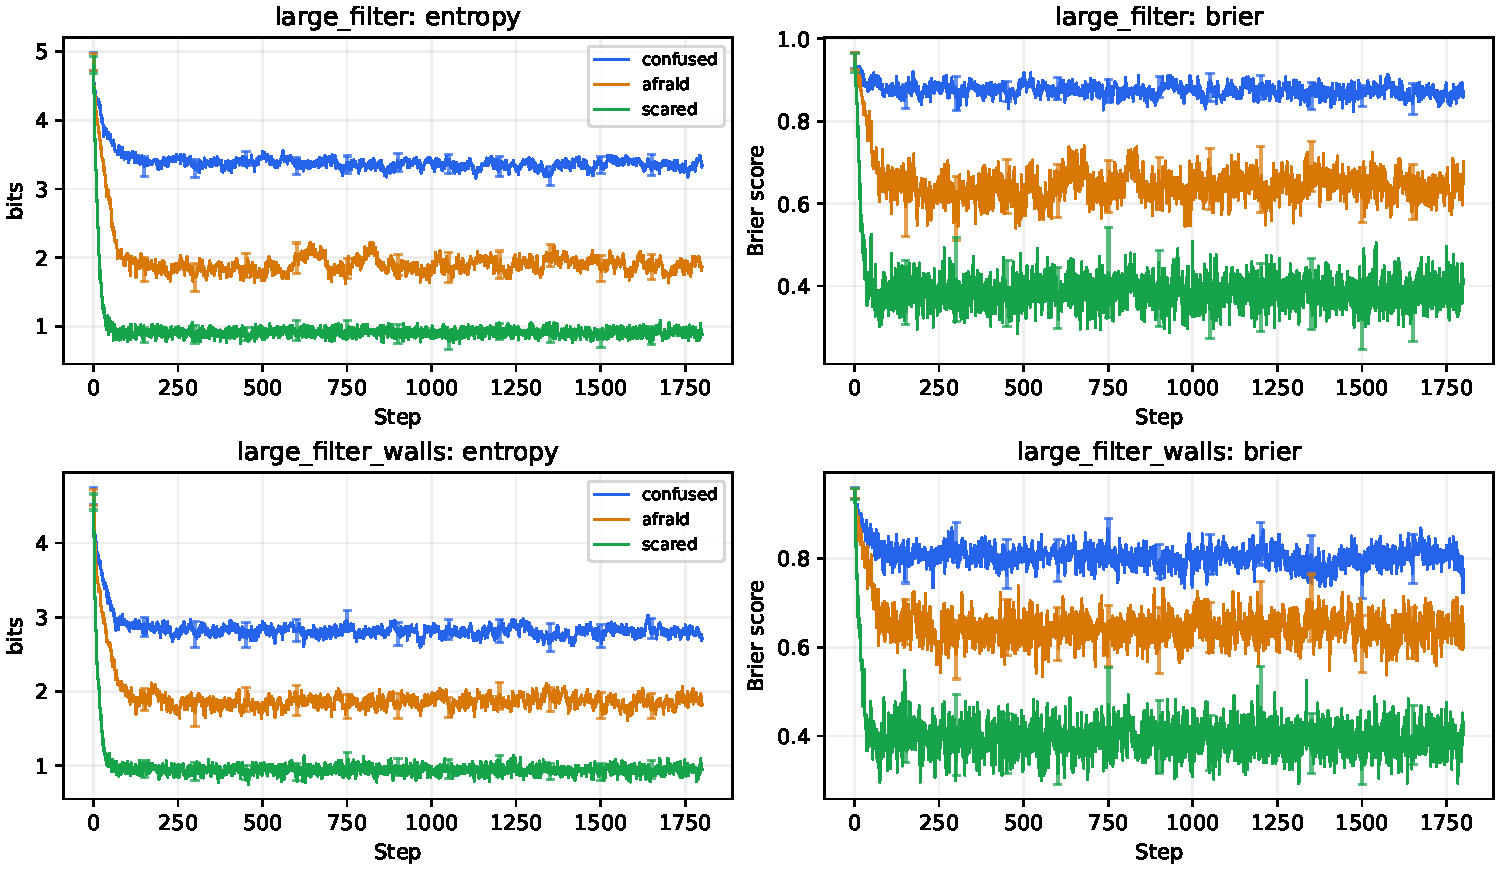
\includegraphics[width=0.94\linewidth]{results/convergence.pdf}
    \end{center}
    Convergence was checked by comparing the final two disjoint windows,
    paired by trial: 600 steps each at $v=0.25,1$, and 3000
    steps each at $v=4$. Across all 18 conditions, the
    largest absolute changes were 0.162 bits and 0.006 Brier units.
    At the required default variance, these maxima were only 0.014
    bits and 0.004 Brier units. The high-noise confused policy still
    shows declining entropy; its variance comparison is a finite-duration
    result, not an equilibrium estimate.
    The raw trial curves, individual confidence intervals and window changes
    are saved in \texttt{results/trials.npz} and \texttt{summary.json}.
    These are empirical stability diagnostics, not a proof of convergence
    for every map or a guarantee of exact localization.

    \item Increasing $q$ makes moves away from Pacman relatively more likely.
    For example, with two approaching and two receding neighbors, the
    probability of a receding move is $1/2$, $2/3$ or $8/9$.
    With a fixed Pacman near a corner, fearful ghosts concentrate near
    distant boundaries or local distance maxima. The measured default-noise
    entropy decreases from confused to afraid to scared in both layouts.
    Walls change available exits and create bottlenecks, so distance-only
    observations interact with map geometry. The table shows the resulting
    uncertainty and accuracy; the ordering does not imply that greater fear
    universally improves inference for arbitrary moving controllers.

    \item Increasing sensor variance broadens the measurement likelihood,
    retaining more plausible positions after each update. The experiment
    below shows greater tail entropy at higher variance for each policy
    on both maps. Transition information remains informative for fearful
    ghosts even when measurements are noisy. Parameter truncation matters:
    only $n/4$ is the actual variance, although the three values tested here
    are represented exactly.
    \begin{center}
    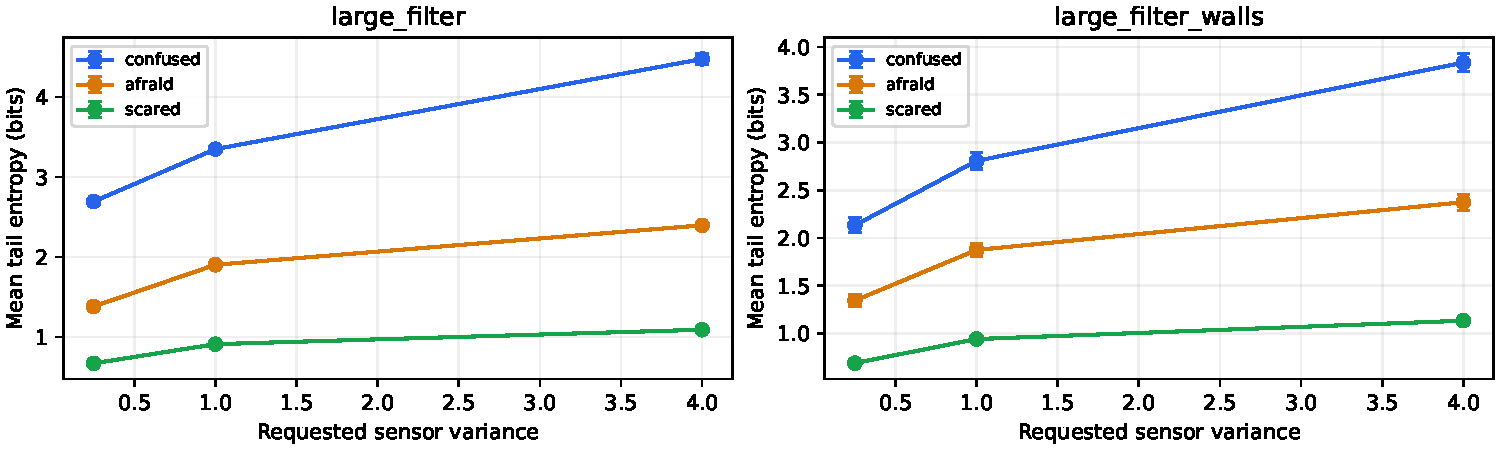
\includegraphics[width=0.94\linewidth]{results/variance.pdf}
    \end{center}

    \item A controller can score legal candidate next cells using their
    capture probability and discounted proximity to belief mass.
    Our controller learns blocked neighbors from legal actions and remembers
    visit counts. Unknown cells remain traversable in its provisional map.
    For each legal move to $z$, it computes provisional maze distances and
    maximizes
    $\sum_g\sum_x b_g(x)e^{-\hat d(z,x)/4}
       +2\sum_g b_g(z)-0.03\,\mathrm{visits}(z)$.
    This favors likely captures and discourages repeated unproductive moves.
    The only state observations are its own position and legal actions;
    neither true ghost coordinates nor the wall-grid accessor is used.
    This is a heuristic controller, with no guarantee of optimal capture time.
    \item \textbf{\textit{Leave empty.}}
\end{enumerate}

% ==============================================================================

\end{document}
